Aplikacja konsolowa do zarządzania domem służy jako aplikacja odpowiedzialna za wszystkie działania związane z Raspberry Pi oraz jego peryferiami. Na te zadania składają się 2 czynności:
\begin{itemize}
\item odczyt wartości sensorów,
\item detekcja ruchu.
\end{itemize}
Obie czynności wykonywane są niezależnie od siebie. Funkcja wykrywania ruchu działa bez przerwy, w przypadku problemu zostanie ponownie uruchomiona po około minucie za pomocą zadania wpisanego do serwisu Crontab. Odczyt parametrów wskazywanych przez czujniki odbywa się cyklicznie co 1 minutę.

\section{Odczyt wartości sensorów}
\begin{figure}[H]
	\centering
	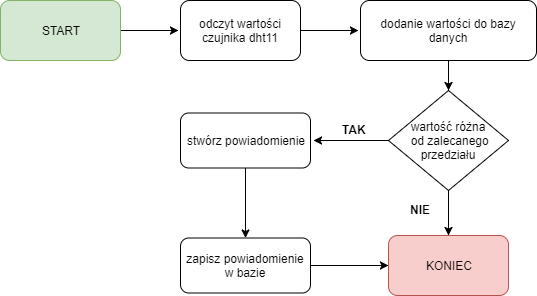
\includegraphics[scale=0.6]{odczyt_czujnikow.png}
	\caption{Proces wykrywania twarzy}
	\label{fig:wykrywanie_proces}
\end{figure}
Proces zbierania danych z sensorów rozpoczyna się od pobrania odczytów z czujnika DHT11. Raspberry komunikuje się z czujnikiem za pomocą protokołu 1-wire. Do pobrania wartości wykorzystano bibliotekę dedykowaną dla tego czujnika i języka Python. Po prawidłowym odczycie, każdy z parametrów (temperatura i wilgotność) zostaje zapisany w bazie danych z odpowiednim opisem. W kolejnym kroku odczytane wartości zostają porównane z wcześniej zdefiniowanym zakresem, który jest zapisany w bazie danych. W przypadku przekroczenia lub zbyt niskiej wartości system podejmie decyzję o utworzeniu nowego powiadomienia, które będzie widoczne an stronie opisanej w rozdziale \ref{notifications}
\section{Detekcja ruchu}

\subsection{Proces wykrywania ruchu}